\documentclass{article}
\usepackage{amsmath}
\usepackage{amsfonts}
\usepackage{amssymb}
\usepackage{amsthm}
\usepackage{geometry}
\usepackage{algorithm}
\usepackage{algpseudocode}
\usepackage{minted}
\usepackage{graphicx}
\usepackage{float}

\geometry{a4paper, left=2cm, right=2cm, top=2cm, bottom=2cm}

\title{Image Processing: Homework 2}
\author{FU, YONG-WEI (112550107)}
\date{\today}

\begin{document}

\maketitle

\section{Part 1: MATLAB Histogram Equalization}
\subsection{Methodology}
For this section, the original color image submitted in Homework 1 was processed using MATLAB. 
First, the image was converted from RGB to grayscale using the \texttt{rgb2gray()} function to 
ensure operations were performed purely on intensity values. Subsequently, the built-in 
\texttt{histeq()} function was utilized. This function computes the cumulative distribution 
function (CDF) of the image's intensity levels and maps the original pixel values to new values 
that are more uniformly distributed across the available intensity range. The result is an image 
with enhanced contrast, where details in darker and lighter regions become more visible. The 
original and equalized images, along with their histograms, were displayed in a 2x2 grid for comparison.
\subsection{Results \& Code}
The following figure displays the original grayscale image on the left, its equalized counterpart on the right, and
their respective histograms on the bottom.

\begin{figure}[H]
    \centering
    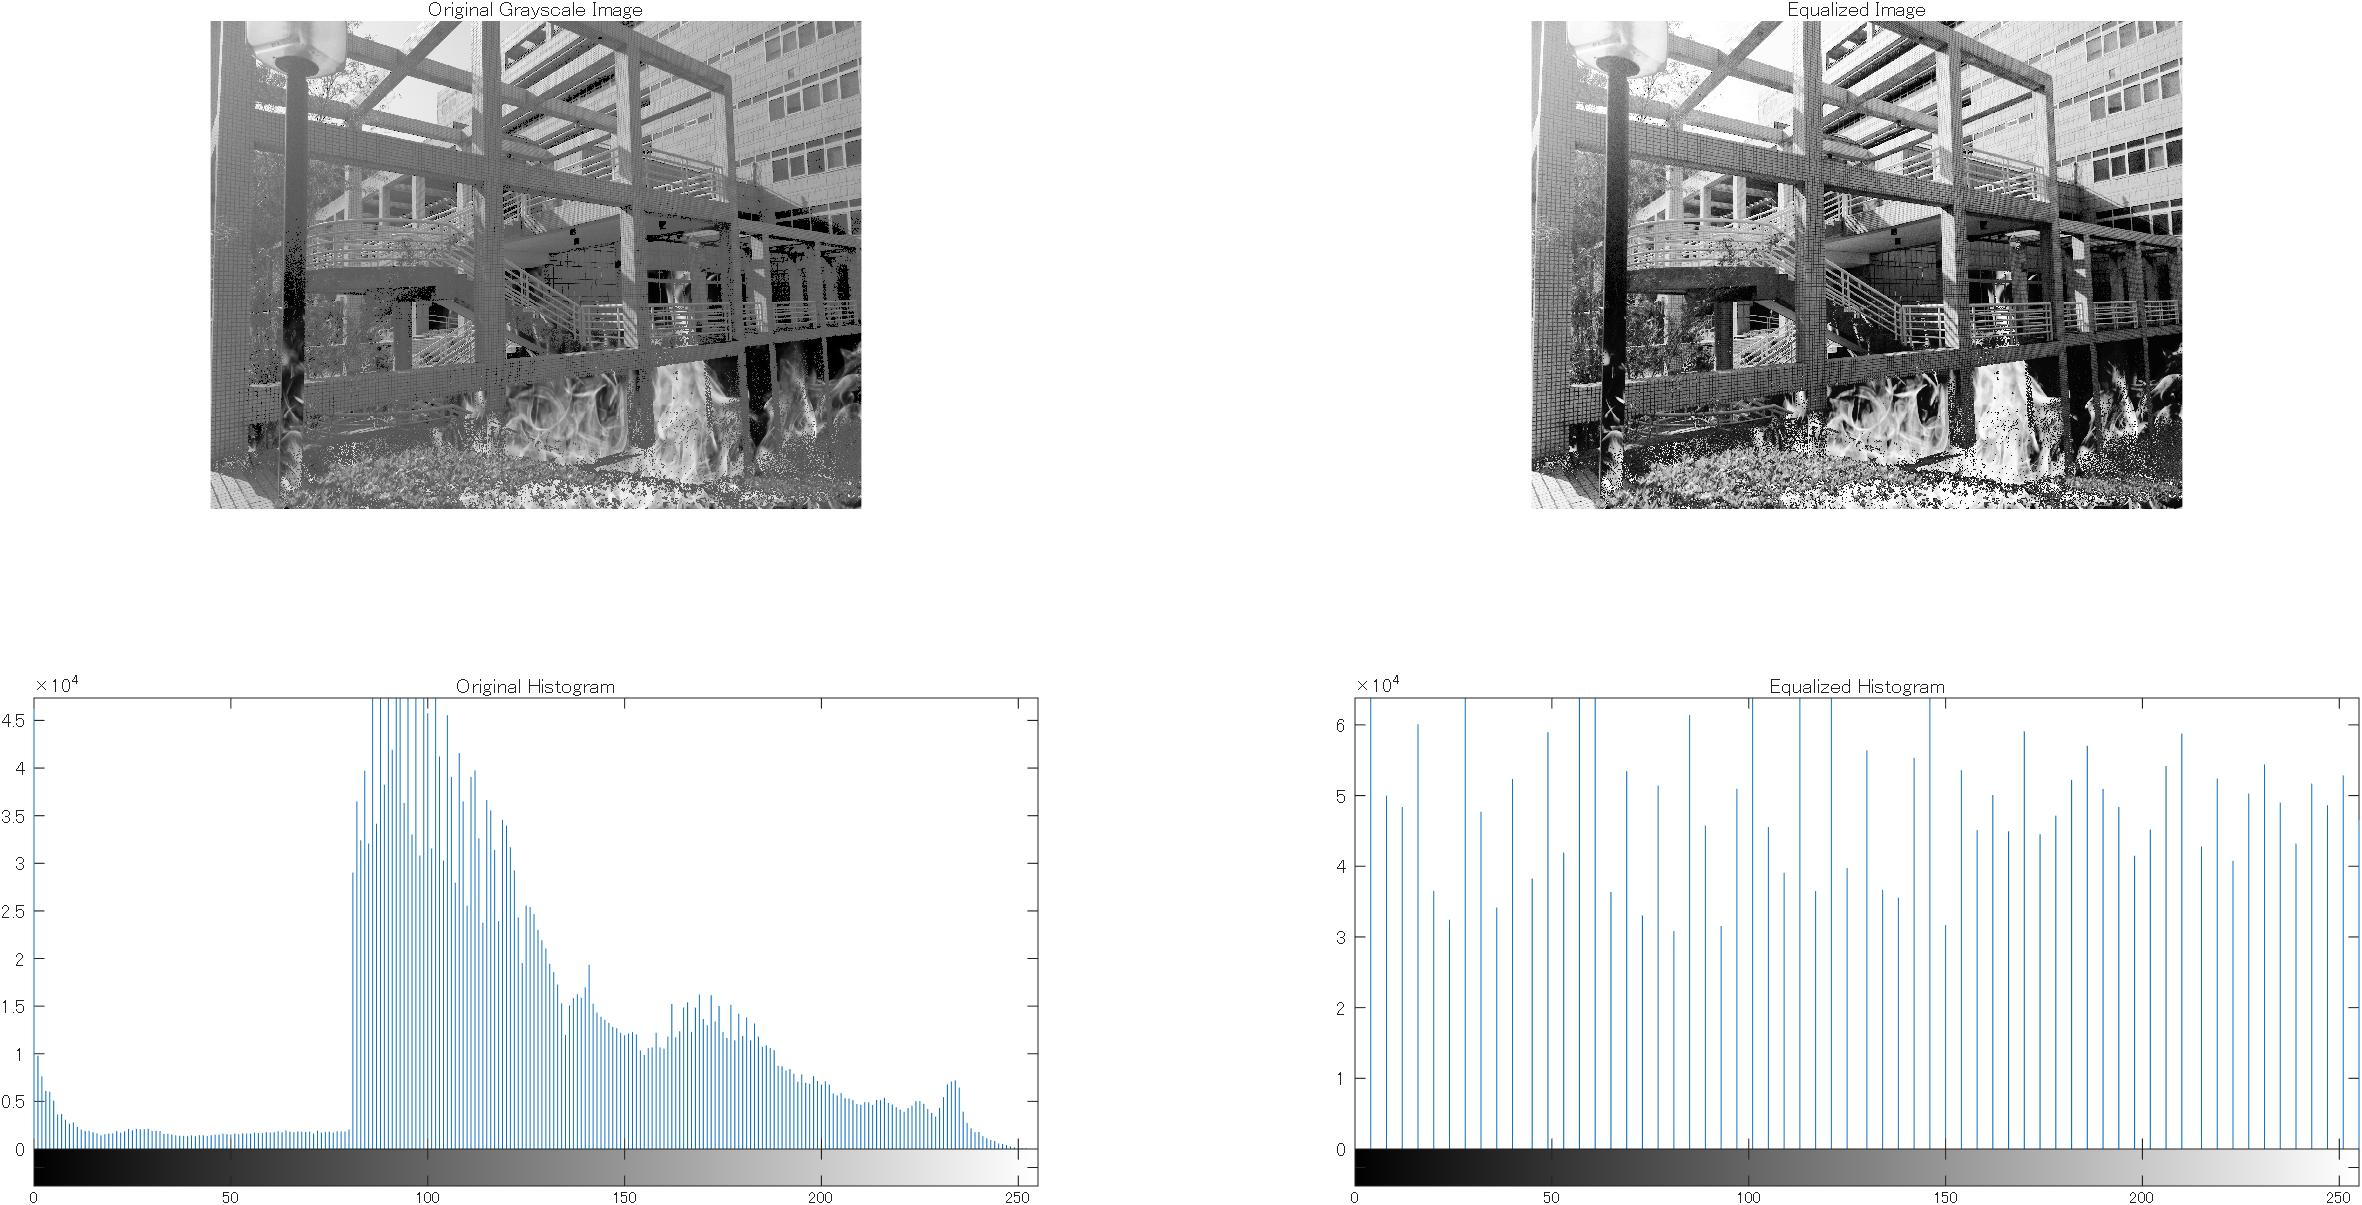
\includegraphics[width=0.9\textwidth]{Q1_matlab/Figure_1.png} 
    \caption{MATLAB Processing: Before and After Equalization}
    \label{fig:matlab}
\end{figure}

The following MATLAB script was used to execute this transformation:

\newpage

\begin{minted}[linenos, breaklines, frame=lines, fontsize=\footnotesize]{matlab}
% Load the original color image
color_img = imread('../../HW1/Q4_Creative_Edit/Q4_final_edit.png');

% Convert the RGB image to grayscale
gray_img = rgb2gray(color_img);

% Perform histogram equalization
eq_img = histeq(gray_img);

% Display the results in a single window
figure;

% Top Left: Original Grayscale Image
subplot(2, 2, 1);imshow(gray_img);title('Original Grayscale Image');

% Top Right: Equalized Image
subplot(2, 2, 2);imshow(eq_img);title('Equalized Image');

% Bottom Left: Original Histogram
subplot(2, 2, 3);imhist(gray_img);title('Original Histogram');

% Bottom Right: Equalized Histogram
subplot(2, 2, 4);imhist(eq_img);title('Equalized Histogram');
\end{minted}

\section{Part 2: Software Histogram Equalization (GIMP)}
\subsection{Methodology}
I chose the open-source program GIMP (GNU Image Manipulation Program) to perform histogram equalization. 
The original image was imported and converted to a grayscale color space. To perform the equalization, 
the built-in tool was accessed via \texttt{Colors > Auto > Equalize}. Similar to the MATLAB function, 
this tool mathematically expands the dynamic range of the image, stretching the clumped mid-range pixel 
intensities across the entire available spectrum.

\subsection{Results}
The following figure displays the original grayscale image on the left, its equalized counterpart after 
the GIMP auto-equalization process on the right, and their respective histograms on the bottom.

\begin{figure}[H]
    \centering
    % Row 1
    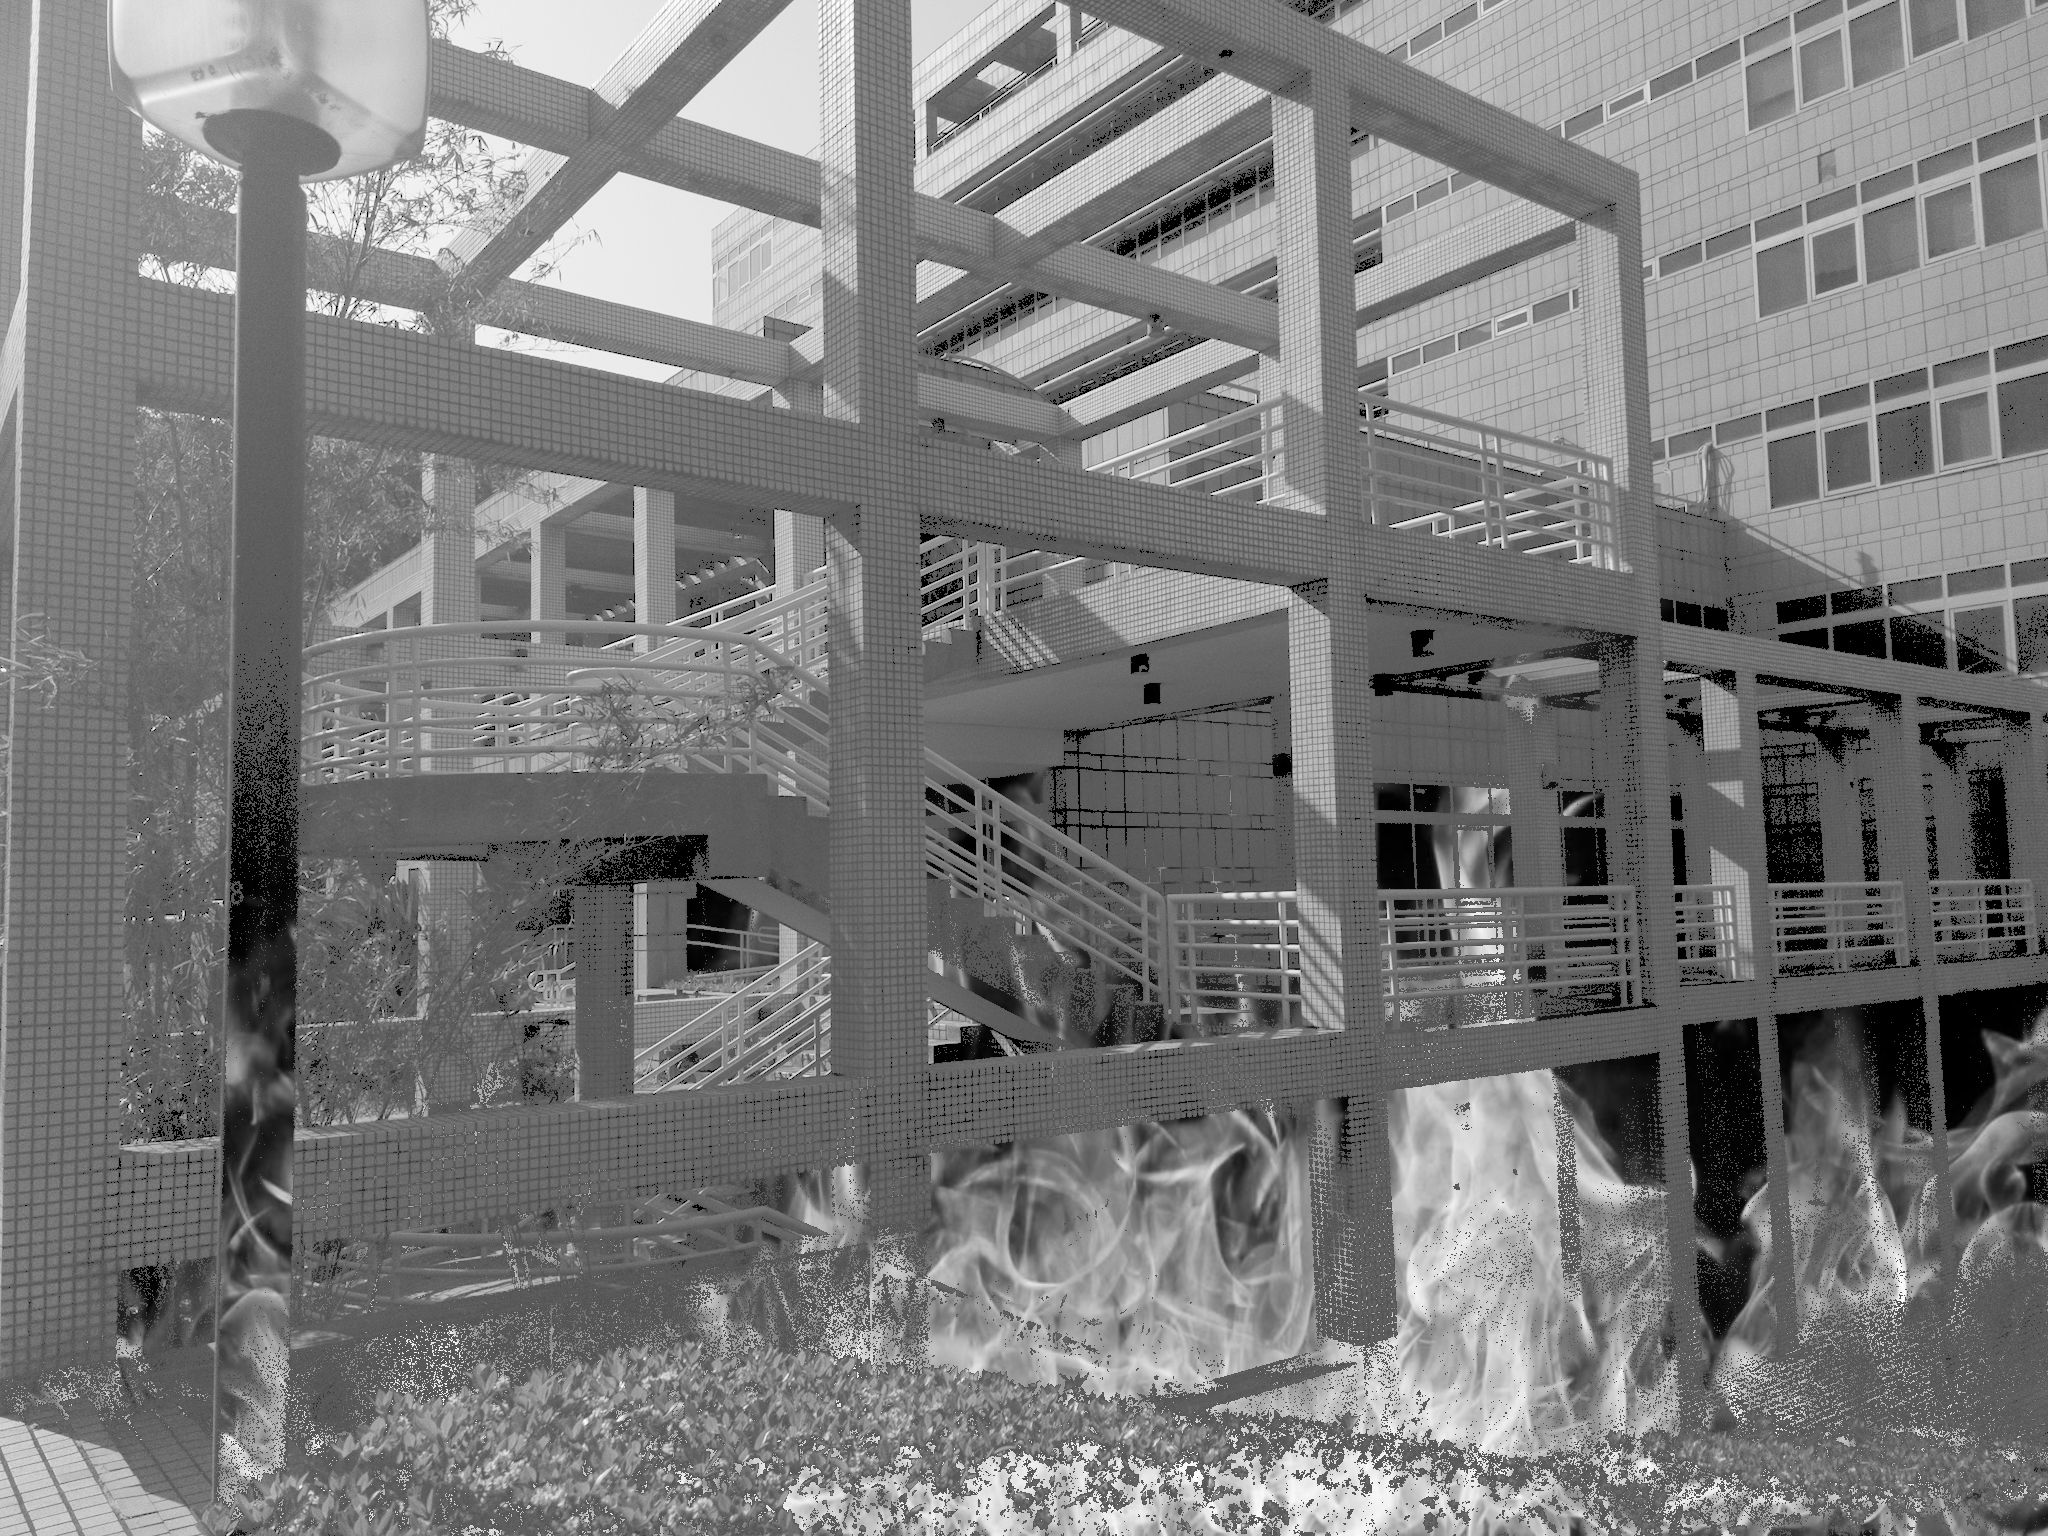
\includegraphics[width=0.4\textwidth]{Q2_GIMP/oriimage.png}
    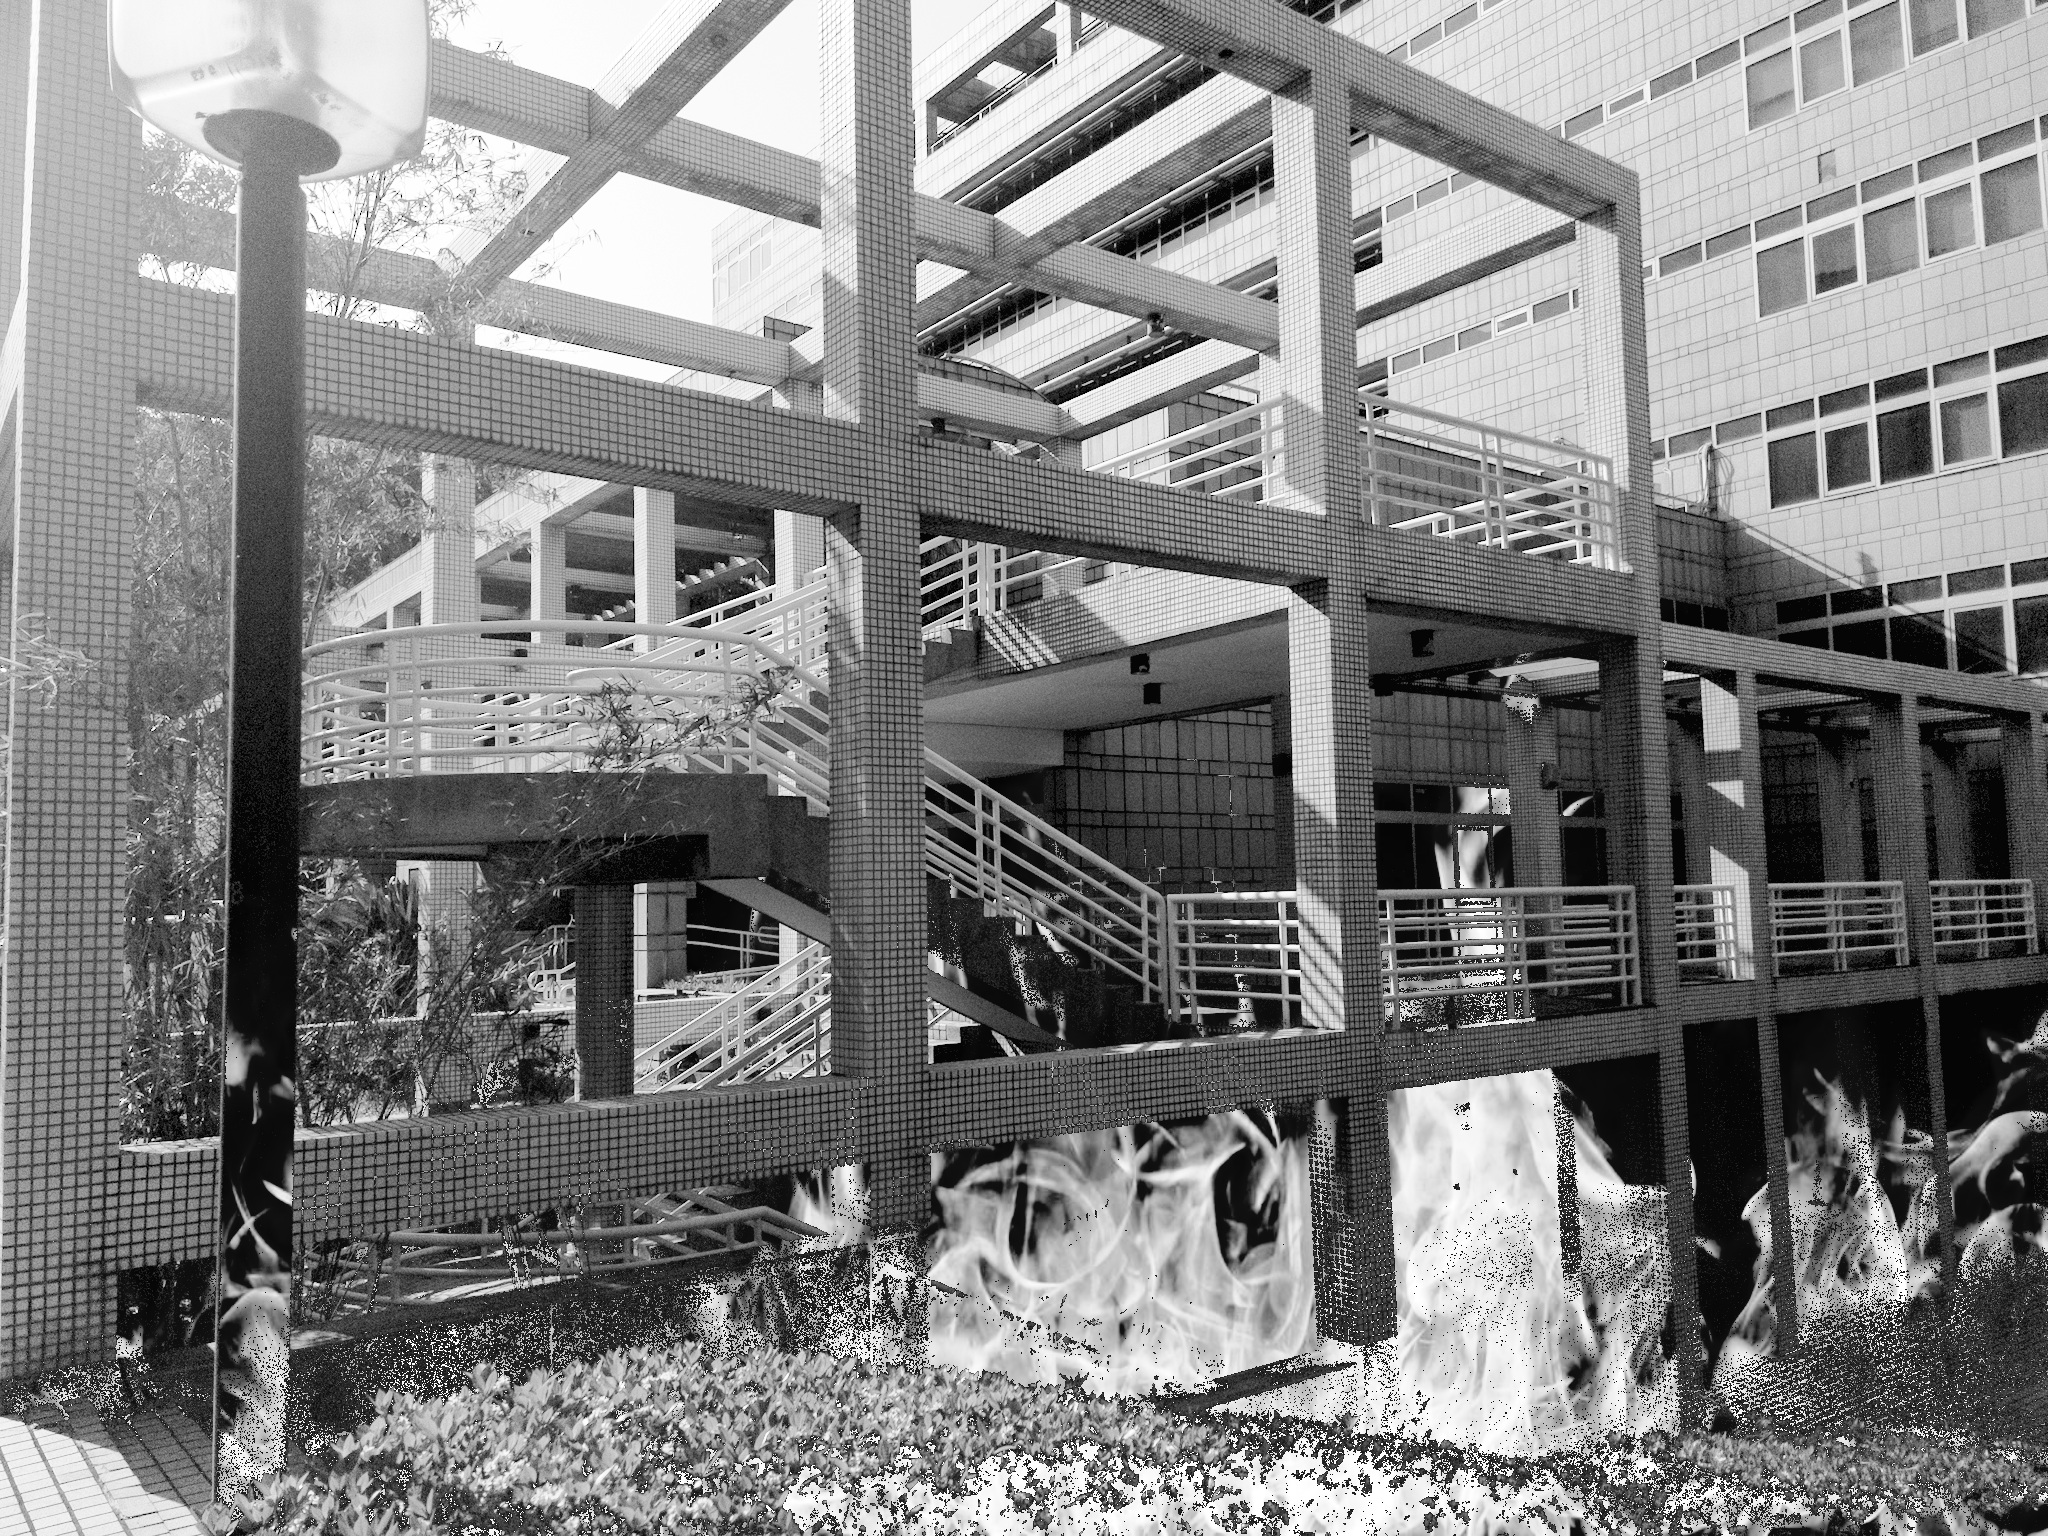
\includegraphics[width=0.4\textwidth]{Q2_GIMP/eqimage.png}
    \\[0.5cm] % Adds a little vertical space between rows
    % Row 2
    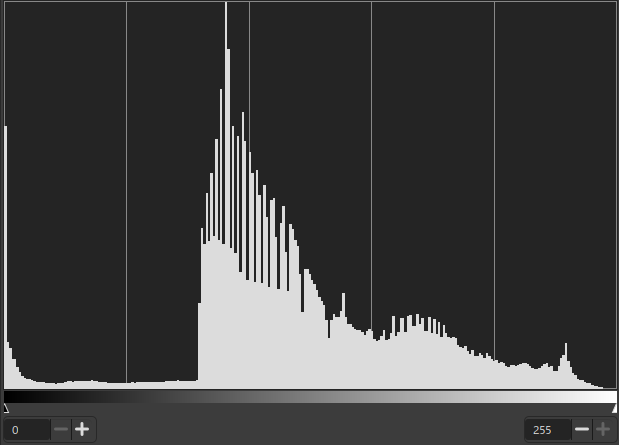
\includegraphics[width=0.4\textwidth]{Q2_GIMP/orihist.png}
    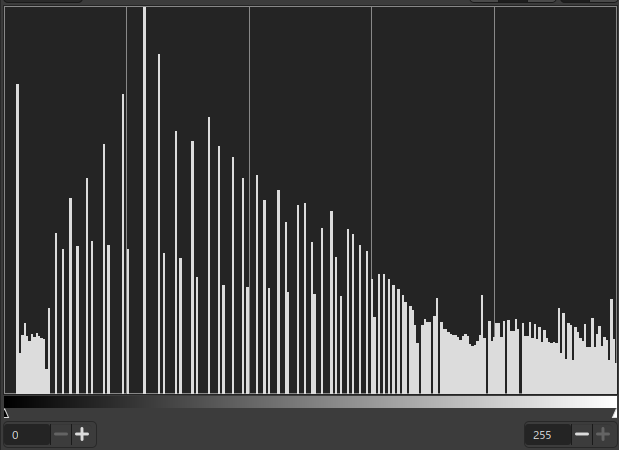
\includegraphics[width=0.4\textwidth]{Q2_GIMP/eqhist.png}
    \caption{GIMP Processing: Before and After Equalization}
    \label{fig:gimp}
\end{figure}

\section{Part 3: Manual Calculations}

\subsection*{(a) Histogram Equalization of Image A}
The equalized pixel values are derived using the CDF. The new mapped value $s_k$ for a 
given intensity level $r_k$ is calculated as $s_k = \text{round}((L-1) \times \text{CDF}(r_k))$.
Given that the image depth is 3 bits, the $L-1$ will be $7$.

\begin{table}[H]
    \centering
    \renewcommand{\arraystretch}{1.2}
    \begin{tabular}{|c|c|c|c|c|}
        \hline
        \textbf{Original Intensity ($r_k$)} & \textbf{Count ($n_k$)} & \textbf{PDF ($p(r_k)$)} & \textbf{CDF} & \textbf{Mapped Output ($s_k$)} \\
        \hline
        0 & 2 & 0.08 & 0.08 & $\text{round}(0.56) = 1$ \\
        1 & 4 & 0.16 & 0.24 & $\text{round}(1.68) = 2$ \\
        2 & 6 & 0.24 & 0.48 & $\text{round}(3.36) = 3$ \\
        3 & 4 & 0.16 & 0.64 & $\text{round}(4.48) = 4$ \\
        4 & 2 & 0.08 & 0.72 & $\text{round}(5.04) = 5$ \\
        5 & 2 & 0.08 & 0.80 & $\text{round}(5.60) = 6$ \\
        6 & 3 & 0.12 & 0.92 & $\text{round}(6.44) = 6$ \\
        7 & 2 & 0.08 & 1.00 & $\text{round}(7.00) = 7$ \\
        \hline
    \end{tabular}
\end{table}

Then, by substituting the original intensity values with their corresponding mapped outputs, we yield the final histogram-equalized intensity matrix for Image A:
\[
A_{eq} = 
\begin{bmatrix}
    3 & 6 & 5 & 7 & 4 \\
    2 & 6 & 3 & 5 & 1 \\
    6 & 3 & 6 & 4 & 7 \\
    4 & 2 & 2 & 3 & 6 \\
    3 & 1 & 3 & 2 & 4 
\end{bmatrix}
\]

\subsection*{(b) Histogram Matching (Image A to Image B)}

\textbf{1. Target Distribution (Image B)}\\
To perform histogram matching, we first determine the target CDF ($C_B$). 

\begin{table}[H]
    \centering
    \renewcommand{\arraystretch}{1.2}
    \begin{tabular}{|c|c|c|c|}
        \hline
        \textbf{Target Intensity ($z_q$)} & \textbf{Count} & \textbf{PDF} & \textbf{Target CDF ($C_B$)} \\
        \hline
        0 & 2 & 0.08 & 0.08 \\
        1 & 4 & 0.16 & 0.24 \\
        2 & 4 & 0.16 & 0.40 \\
        3 & 3 & 0.12 & 0.52 \\
        4 & 3 & 0.12 & 0.64 \\
        5 & 3 & 0.12 & 0.76 \\
        6 & 4 & 0.16 & 0.92 \\
        7 & 2 & 0.08 & 1.00 \\
        \hline
    \end{tabular}
\end{table}

\vspace{1em}
\textbf{2. CDF Mapping Calculation}\\
We map each original intensity level $r_k$ from Image A to a new intensity level $z_q$ in Image B by finding the value where the Target CDF ($C_B$) most closely matches the Input CDF ($C_A$).

\begin{table}[H]
    \centering
    \renewcommand{\arraystretch}{1.2}
    \begin{tabular}{|c|c|c|c|}
        \hline
        \textbf{Original $r_k$} & \textbf{Input CDF ($C_A$)} & \textbf{Closest Target CDF ($C_B$)} & \textbf{Mapped Output ($z_q$)} \\
        \hline
        0 & 0.08 & 0.08 & 0 \\
        1 & 0.24 & 0.24 & 1 \\
        2 & 0.48 & 0.52 & 3 \\
        3 & 0.64 & 0.64 & 4 \\
        4 & 0.72 & 0.76 & 5 \\
        5 & 0.80 & 0.76 & 5 \\
        6 & 0.92 & 0.92 & 6 \\
        7 & 1.00 & 1.00 & 7 \\
        \hline
    \end{tabular}
\end{table}

\vspace{1em}
\textbf{3. Final Intensity Matrix}\\
Applying this intensity mapping to the original spatial arrangement of Image A yields the final histogram-matched matrix:
\[
A_{matched} = \begin{bmatrix}
3 & 6 & 5 & 7 & 4 \\
1 & 5 & 3 & 5 & 0 \\
6 & 3 & 5 & 4 & 7 \\
4 & 1 & 1 & 3 & 6 \\
3 & 0 & 3 & 1 & 4 
\end{bmatrix}
\]

\subsection*{(c) Laplacian Sharpening at Center Pixel}

\textbf{1. Target Extraction}\\
The center pixel of Image A is located at coordinate (2,2) with an original intensity of $f(2,2) = 5$. 
To calculate the Laplacian at this position, we extract the $3\times3$ neighborhood surrounding it:
\[
\text{Neighborhood} = \begin{bmatrix}
5 & 2 & 4 \\
2 & \mathbf{5} & 3 \\
1 & 1 & 2 
\end{bmatrix}
\]

\vspace{1em}
\textbf{2. Laplacian Calculation}\\
We apply the provided $3\times3$ Laplacian kernel to this neighborhood by computing the sum of the element-wise products:
\[
\nabla^2 f(2,2) = \sum_{i=-1}^{1} \sum_{j=-1}^{1} \text{Neighborhood}(i,j) \cdot \text{Kernel}(i,j)
\]
\[
\nabla^2 f(2,2) = (2 \times -1) + (2 \times -1) + (5 \times 4) + (3 \times -1) + (1 \times -1)
\]
\[
\nabla^2 f(2,2) = -2 - 2 + 20 - 3 - 1 = 12
\]

\vspace{1em}
\textbf{3. Sharpening and Clipping}\\
Because the center weight of the given Laplacian kernel is positive, the sharpened image $g(x,y)$ is obtained by 
adding the Laplacian result back to the original image:
\[
g(2,2) = f(2,2) + \nabla^2 f(2,2) = 5 + 12 = 17
\]
However, the problem specifies that the image depth is 3 bits. Therefore, the maximum allowable intensity 
is $2^3 - 1 = 7$. Since 17 exceeds this dynamic range, the value must be clipped to the maximum limit, which will be 7.

\subsection*{(d) Highboost Filtering at Center Pixel}

\textbf{1. Original and Blurred Values}\\
The original intensity of the center pixel of Image A is $f(2,2) = 5$. 
The blurred image $\bar{f}(x,y)$ is generated using a $5\times5$ box kernel. 
Because the center pixel's $5\times5$ neighborhood encompasses the entirety of Image A, 
the blurred value is the arithmetic mean of all 25 pixels in the image, which is 78.
\[
\bar{f}(2,2) = \frac{1}{25} \sum_{i=0}^{4} \sum_{j=0}^{4} A(i,j) = \frac{78}{25} = 3.12
\]

\vspace{1em}
\textbf{2. Unsharp Mask Extraction}\\
The mask, which isolates the high-frequency details, is obtained by subtracting the blurred value 
from the original intensity:
\[
g_{mask}(2,2) = f(2,2) - \bar{f}(2,2) = 5 - 3.12 = 1.88
\]

\vspace{1em}
\textbf{3. Highboost Calculation and Clipping}\\
Using the highboost factor $k=3$, the final filtered value $g(x,y)$ is calculated by adding the 
scaled mask back to the original pixel:
\[
g(2,2) = f(2,2) + k \cdot g_{mask}(2,2)
\]
\[
g(2,2) = 5 + 3(1.88) = 5 + 5.64 = 10.64
\]
Rounding this result to the nearest integer yields 11. However, because the image depth is constrained 
to 3 bits, the maximum possible intensity is $2^3 - 1 = 7$. As the calculated value exceeds the dynamic 
range, it must be clipped to the maximum limit, resulting in a final value of 7.

\subsection*{(e) Full Convolution of Image A}

\textbf{1. Kernel Rotation and Padding}\\
By definition, convolution requires the $3\times3$ kernel $W$ to be rotated 180 degrees prior to application:
\[
W = \begin{bmatrix}
0.1 & 0.2 & 0.3 \\
0.2 & 1.0 & 0.2 \\
0.3 & 0.2 & 0.1 
\end{bmatrix} \quad \xrightarrow{\text{Rotate } 180^{\circ}} \quad W' = \begin{bmatrix}
0.1 & 0.2 & 0.3 \\
0.2 & 1.0 & 0.2 \\
0.3 & 0.2 & 0.1 
\end{bmatrix}
\]

To perform a \textit{full} convolution, Image A must be zero-padded. The required padding size is $K - 1 = 2$ on all 
borders. Applying a $3\times3$ kernel to a $5\times5$ image yields an output matrix of size $(M+K-1) \times (N+K-1) = 7\times7$.

\vspace{1em}
\textbf{2. Output Matrix Calculation}\\
Sliding the kernel $W'$ over the padded Image A and computing the sum of the element-wise products for all 49 positions 
yields the following full convolution matrix:

\[
C = \begin{bmatrix}
0.2 & 1.0 & 2.2 & 3.3 & 2.9 & 2.7 & 0.9 \\
0.5 & 3.9 & 8.7 & 8.9 & 9.8 & 3.2 & 0.9 \\
1.4 & 5.6 & 10.9 & 9.2 & 9.9 & 4.4 & 2.4 \\
1.8 & 8.4 & 7.1 & 8.8 & 7.7 & 9.8 & 3.2 \\
2.6 & 5.8 & 4.9 & 4.0 & 6.9 & 5.0 & 2.0 \\
1.3 & 3.2 & 2.7 & 2.5 & 4.1 & 3.8 & 0.8 \\
0.6 & 0.4 & 0.8 & 0.9 & 1.2 & 0.7 & 0.3
\end{bmatrix}
\]

\subsection*{(f) Full Correlation of Image A}
Because $W = W'$, the convolution operation for this specific kernel is mathematically identical to cross-correlation. 
Therefore, the full correlation yields the exact same $7\times7$ output matrix as the full convolution:
\[
\text{Correlation Matrix} = C 
\]

\subsection*{(g) Bilinear Interpolation at Position (2.5, 1.5)}

\textbf{1. Identify Surrounding Coordinates}\\
The target position $(2.5, 1.5)$ is bounded by the following four integer coordinates in Image A:
\begin{itemize}
    \item Top-Left $(x_1, y_1) = (2, 1) \rightarrow f(2,1) = 2$
    \item Top-Right $(x_2, y_1) = (3, 1) \rightarrow f(3,1) = 4$
    \item Bottom-Left $(x_1, y_2) = (2, 2) \rightarrow f(2,2) = 5$
    \item Bottom-Right $(x_2, y_2) = (3, 2) \rightarrow f(3,2) = 3$
\end{itemize}

\vspace{1em}
\textbf{2. Horizontal Interpolation (X-Axis)}\\
We perform linear interpolation along the x-axis for both the top and bottom rows. 
Since $x=2.5$ is exactly the midpoint between $x_1=2$ and $x_2=3$, the interpolated values are simply the arithmetic means:
\[
f(2.5, 1) = 0.5 \cdot f(2,1) + 0.5 \cdot f(3,1) = 0.5(2) + 0.5(4) = 3
\]
\[
f(2.5, 2) = 0.5 \cdot f(2,2) + 0.5 \cdot f(3,2) = 0.5(5) + 0.5(3) = 4
\]

\vspace{1em}
\textbf{3. Vertical Interpolation (Y-Axis) and Rounding}\\
Next, we interpolate vertically between our two newly calculated horizontal midpoints. 
Since $y=1.5$ is the midpoint between $y_1=1$ and $y_2=2$:
\[
f(2.5, 1.5) = 0.5 \cdot f(2.5, 1) + 0.5 \cdot f(2.5, 2) = 0.5(3) + 0.5(4) = 3.5
\]
Because the image is constrained to a 3-bit depth, pixel intensities must be discrete integers. 
Rounding $3.5$ to the nearest integer yields the final interpolated intensity, which is 4.

\end{document}